\section{Ergebnisse}
\label{sec:ergebnisse}
Dieses Kapitel widmet sich den Ergebnissen dieser Arbeit. 
Im Kap.~\ref{subsec:ablauf} wurde eine grobe Schilderung gegeben, wie die Pipeline aussieht, die ein beliebiges 3D-Modell durchläuft, bis es gezeichnet wird.
Im ersten Anlauf wurde ein Datensatz bestehend aus 11 unterschiedlichen 3D-Modellen durch diese Pipeline geschickt. 
Dabei wurde der Kompressionsstandard Brotli-G untersucht. 
Wichtige Gesichtspunkte für die Auswertung sind das Kompressionsverhältnis, und die Geschwindigkeit, in der die komprimierten Dreiecksnetze dekomprimiert werden. 
Die visuelle Qualität muss im ersten Anlauf zwangsweise unverändert bleiben, da Brotli-G verlustfrei komprimiert (Kap.~\ref{subsec:brotli}). 
Die Ergebnisse des ersten Ablaufs sind in der nachfolgenden Abb.(einfügen) dokumentiert.

\begin{figure}[htb]
  \centering  
  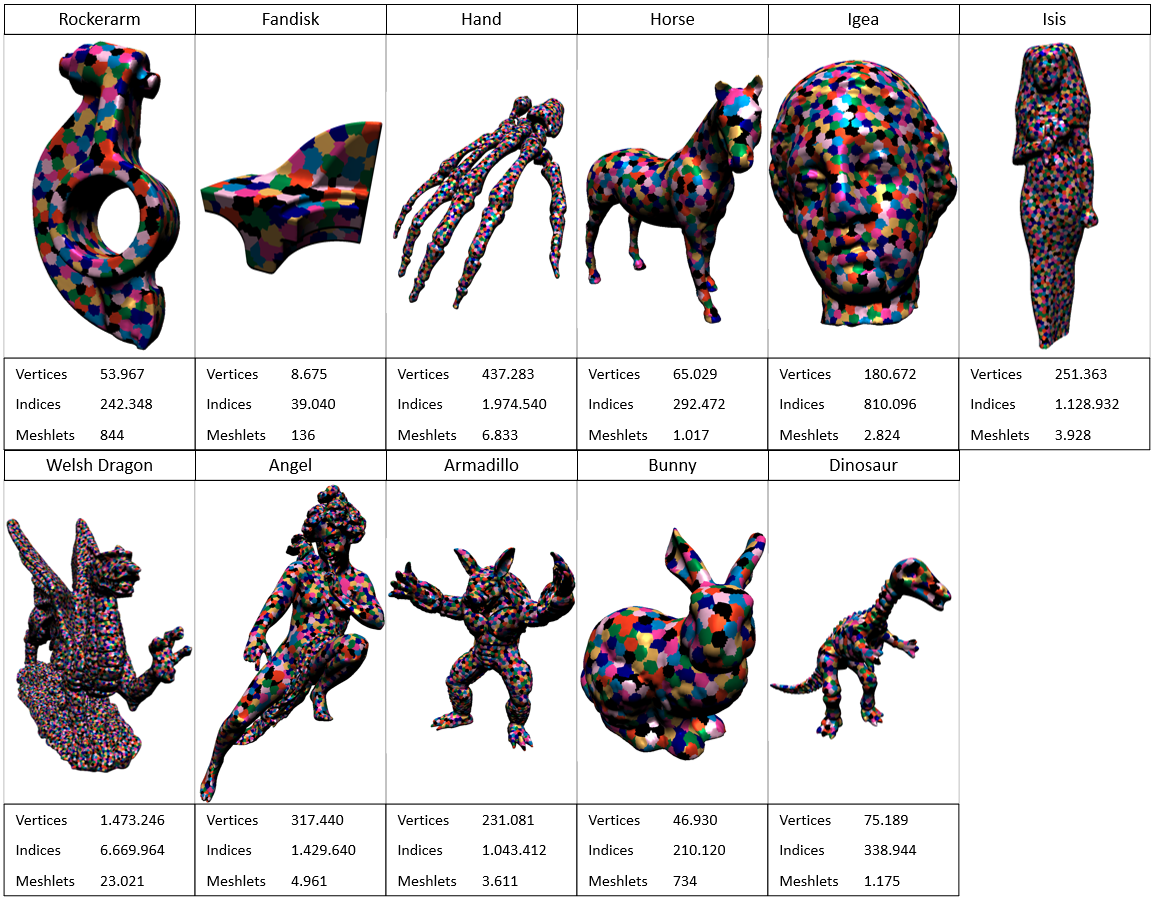
\includegraphics[scale=0.5]{Bilder/Ergebnisse_zusammen.png}
  \caption[Der verwendete Datensatz]{\textbf{Der verwendete Datensatz} Die Abbildung zeigt alle Dreiecksnetze mit der Anzahl an Vertices/Indizes/Meshlets. }
  \label{fig:mesh_shading_pipeline}
\end{figure}

Der Datensatz besteht aus vielen unterschiedlichen 3D-Modellen unterschiedlicher Größe. 
Von einem sehr kleinem Modell der „Fandisk“ mit 136 Meshlets, bis hin zu einem „Welsh Dragon“, der aus ganzen 23.021 Meshlets besteht, werden nun die Ergebnisse des Brotli-G Kodierers ausgewertet und analysiert.

\subsection{Auswertung des Datensatzes}
\label{subsec:auswertung1}
Betrachten wir zunächst das Dreiecksnetz mit der geringsten Anzahl an Vertices/Indizes/Meshlets. 
Die Ergebnisse des Kodierers sind sehr vielversprechend. 
Die 366.536 Bytes des Originalmodells komprimiert Brotli-G auf 160.200 Bytes, und erreicht somit ein Kompressionsverhältnis von 2,29.
Auffällig sind hierbei jedoch die Dekompressionszeiten für dieses sehr kleine Modell. 
Bei der Größe des Modells und der doch sehr hohen Dekompressionszeit für den GPU Dekodierer wird eine Bandbreite von 0,054 GiB/s erreicht, was deutlich weniger ist, als was der PCIE-Bus der GPU zulässt, die für den Versuch verwendet wurde.

\begin{figure}[htb]
  \centering  
  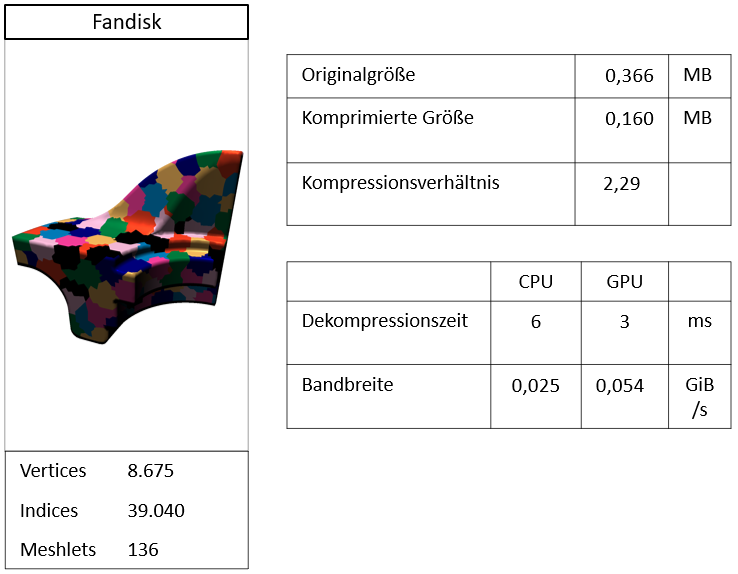
\includegraphics[scale=0.75]{Bilder/ergebnisse/fandisk.png}
  \caption[Fandisk Kompressionsergebnis]{\textbf{Fandisk Kompressionsergebnis} Das kleinste Dreiecksnetz aus dem Datensatz, und seine Ergebnisse}
  \label{fig:mesh_shading_pipeline}
\end{figure}

Um die niedrige Bandbreite zu erklären, können die Ergebnisse des Welsh Dragons betrachtet werden. 
Dieser besteht aus sehr viel mehr Vertices/Indizes/Meshlets, was sich in der Größe des Modells widerspiegelt. 
Der Welsh Dragon hat eine Originalgröße von 62406096 Bytes, die auf 31716764 Bytes komprimiert wurde. 
Das entspricht einem Kompressionsverhältnis von 1,97.
Viel interessanter hierbei sind jedoch die Dekompressionszeit und die daraus resultierende Bandbreite. 
Der GPU Brotli-G GPU Dekodierer benötigt nicht unbedingt viel mehr Zeit für den Welsh Dragon (7 ms) gegenüber der Fandisk (3 ms).
Bei Anbetracht der komprimierten Größe der beiden Dreiecksnetze fällt auf, das der Welsh Dragon sehr viel mehr Daten benötigt. 
Während die Dekompression des Welsh Dragons etwas mehr als das zweifache der Zeit der Fandisk benötigt, ist die komprimierte Größe des Welsh Dragons etwa 200x so groß wie diese.
Das Ergebnis davon ist in der Bandbreite zu sehen, die beim Welsh Dragon sehr viel besser ist, jedoch noch immer sehr weit von den gewünschten Werten entfernt ist.
Die parallele Dekodierung des Brotli-G Dekodierers scheint daher erst bei größeren Datensätzen richtig effektiv zu werden.

\begin{figure}[htb]
  \centering  
  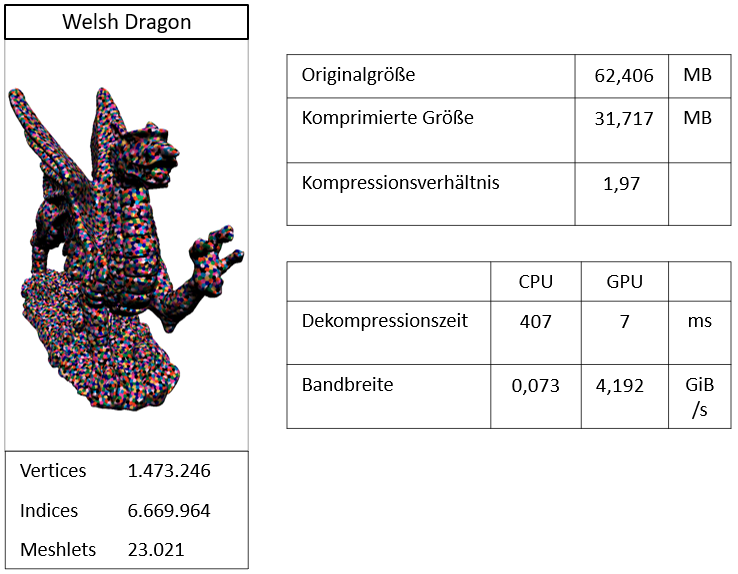
\includegraphics[scale=0.75]{Bilder/ergebnisse/welshdragon.png}
  \caption[Welsh Dragon Kompressionsergebnis]{\textbf{Welsh Dragon Kompressionsergebnis} Das größte Dreiecksnetz aus dem Datensatz, und seine Ergebnisse}
  \label{fig:mesh_shading_pipeline}
\end{figure}

\subsection{Auswertung der quantisierten Vertex-Daten}
\label{subsec:auswertung2}
Im zweiten Anlauf werden die Vertex Daten vor der Komprimierung zu 16-Bit floating point values quantisiert.
Ziel davon ist, die niederwertigen Bits, die nur noch wenig zur Struktur des 3D-Modells beitragen, loszuwerden.
Die hinteren 16 Bit einer 32 Bit Gleitkommazahl beansprucht genausoviel Speicher wie die vorderen 16 Bit.
Während die vorderen Bits jedoch die grobe Position des Vertex, oder auch die Richtung der Normalen, sind die niederwertigen Bits für sehr feine details wichtig.
Wenn es jedoch nicht gerade in Richtung von medizinischen Anwendungen geht, oder allgemeiner beschrieben in Bereiche, in denen diese feine Granularität sehr wichtig ist, sind 16 Bit pro Komponente ausreichend, damit ein Dreiecks visuell ansprechend bleibt. \newline

Um die Qualität zu visualisieren, sieht man in Abb.~\ref{fig:bunny} das Stanford Bunny einmal mit 16, und einmal mit 32 Bit Vertex Attributen.

\begin{figure}[htb]
  \centering  
  \includegraphics[scale=0.45]{Bilder/bunny_quantisiert.png}
  \caption[Quantisiertes Stanford Bunny]{\textbf{Quantisiertes Stanford Bunny} Die Abbildung zeigt eine Gegenüberstellung des Bunnys mit 32 Bit Vertex Attributen und dem Bunny mit den quantisierten 16 Bit Vertex Attributen }
  \label{fig:bunny}
\end{figure}

Bei der Gegenüberstellung sind die Unterschiede kaum erkennbar, was sehr hilfreich ist, wenn die Kompression mit Brotli-G betrachtet wird.
Um einen Vergleich der Ergebnisse zu ziehen wird wieder der Welsh Dragon zur Auswertung der Kompressionsergebnisse verwendet.
Lediglich die Quantisierung der Vertex Daten spart rund 29\% der Größe vor der Komprimierung.
Die Originalgröße von 44.727.144 Bytes wird anschließend von Brotli-G auf 17.260.728 Bytes komprimiert, was einem Kompressionsverhältnis von 2,59 entspricht.
Die Dekomprimierung auf der GPU nimmt mit 6 ms in etwa soviel Zeit in Anspruch wie der Welsh Dragon mit 32 Bit Gleitkommazahlen.
Dadurch ergibt sich eine Bandbreite von $\mathit{2,706 \ GiB/s}$. \newline

Im Anhang sind die Ergebnisse für alle Dreiecksnetze aus dem Datensatz ersichtlich.
Dabei fällt auf, das der Welsh Dragon bei der Betrachtung der Kompressionsverhältnisse kein Einzelfall ist.
Betrachtet man die Ergebnisse von quantisierten und nicht quantisierten Dreiecksnetzen, ist klar zu erkennen, das die quantisierten Dreiecksnetze nicht nur weniger Speicherplatz beanspruchen.
Das Kompressionsverhältnis ist im Durchschnitt des Datensatzes bei den quantisierten Dreiecksnetzen um $\mathit{18,82\%}$.

\begin{figure}[htb]
  \centering  
  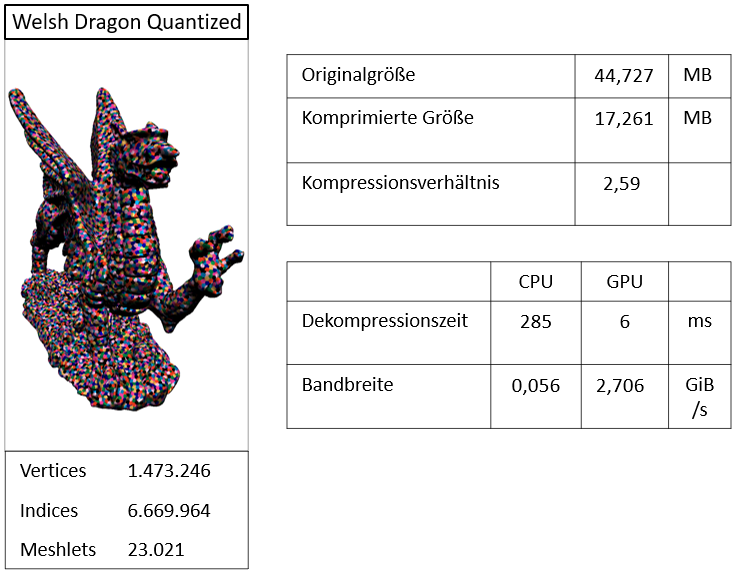
\includegraphics[scale=0.75]{Bilder/ergebnisse/welshdragon_q.png}
  \caption[Welsh Dragon Kompressionsergebnis quantisiert]{\textbf{Welsh Dragon Kompressionsergebnis quantisiert} Die Ergebnisse des quantisierten Welsh Dragon }
  \label{fig:quantized_welsh_dragon}
\end{figure}

\subsection{Auswertung eines großen Dreiecksnetzes}
\label{subsec:auswertung3}
Wie in den anderen Versuchen erkannt wurde, wird eine bestmögliche Bandbreite bei großen Dreiecksnetzen erreicht.
Dafür wird in diesem Abschnitt ein Teil eines großen Dreiecksnetzes des Davids ausgewertet.
Leider legt Brotli-G eine maximale GPU Buffer Größe von 1 GB fest, wodurch ein maximal zu dekodierender Block eingeschränkt wird.
Sollte ein größeres Dreiecksnetz dekodiert werden, muss dieses sinngemäß zugeschnitten werden.
Die Haare des David bestehen aus fünf kleinen Teilstücken, die zusammengetragen eine Größe von rund 760 MB aufweisen, und so einen Großteil der maximalen Buffergröße verwenden.
Die kleinen Teilstücke wurden auf der CPU nacheinander eingelesen, und in ein gemeinsames Binärobjekt geschrieben, das von Brotli-G kodiert worden ist. \newline
Brotli-G hat die Größe des Davids von 759.567.128 Bytes auf 326.929.888 Bytes komprimiert, und somit ein Kompressionsverhältnis von 2,32 erreicht.
Auf der GPU wurde dieses in 65 ms dekomprimiert, wodurch eine Bandbreite von $\mathit{4,682 \ GiB/s}$ erreicht wurde.

\begin{figure}[htb]
  \centering  
  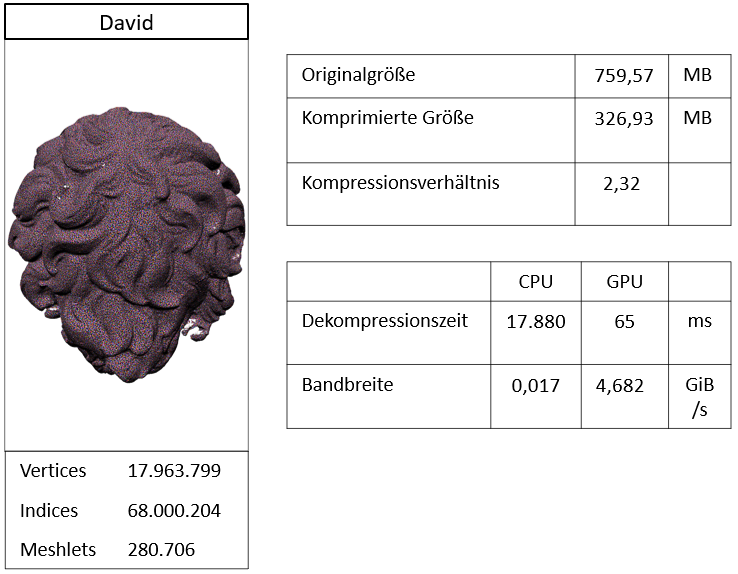
\includegraphics[scale=0.75]{Bilder/ergebnisse/david.png}
  \caption[David Kompressionsergebnis]{\textbf{David Kompressionsergebnis} Ein Teil von dem großen Dreiecksnetzes des Davids }
  \label{fig:david_ergebnis}
\end{figure}

Auch bei diesem Dreiecksnetz wird zusätzlich noch ein Ergebnis mit quantisierten Vertex Attributen durchgeführt.
Durch die Quantisierung der Vertex Attribute kann beim David etwas mehr als 200 MB an Speicher reduzieren.


\begin{figure}[htb]
  \centering  
  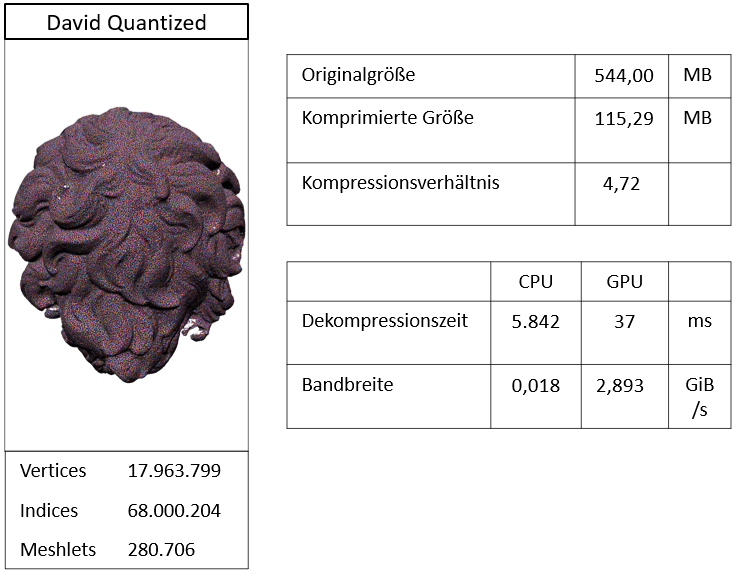
\includegraphics[scale=0.75]{Bilder/ergebnisse/david_q.png}
  \caption[David Kompressionsergebnis quantisiert]{\textbf{David Kompressionsergebnis quantisiert} Ein Teil von dem großen Dreiecksnetzes des Davids mit quantisierten Vertex Attributen }
  \label{fig:david_ergebnis}
\end{figure}

Das Kompressionsverhältnis des quantisierten Davids ist mit 4,67 sehr gut, und dadurch zurückzuführen, das der Scan sehr detailiert 